\documentclass[conference]{IEEEtran}
\IEEEoverridecommandlockouts
% The preceding line is only needed to identify funding in the first footnote. If that is unneeded, please comment it out.
\usepackage{cite}
\usepackage{amsmath,amssymb,amsfonts}
\usepackage{algorithmic}
\usepackage{graphicx}
\usepackage{textcomp}
\usepackage{xcolor}
\usepackage{enumitem}
\def\BibTeX{{\rm B\kern-.05em{\sc i\kern-.025em b}\kern-.08em
    T\kern-.1667em\lower.7ex\hbox{E}\kern-.125emX}}
\begin{document}

\title{Literature Survey: Dynamic Memory Optimization of Serverless Function using RL/ML\\
{\footnotesize CS598 Cloud Computing Capstone Project (CCC) Fall 2023}
\thanks{University of Illinois, Urbana-Champaign.}
}

\author{\IEEEauthorblockN{Hao Zhang}
\IEEEauthorblockA{haoz18@illinois.edu}
\and
\IEEEauthorblockN{Yunxuan Li}
\IEEEauthorblockA{yunxuan6@illinois.edu}
\and
\IEEEauthorblockN{Cesar Arevalo}
\IEEEauthorblockA{cesara2@illinois.edu}
}

\maketitle

\section{Project Idea}
Our goal is to design and implement a framework that can automatically find and apply the optimal resource configuration for serverless functions in the fly, with the adoption of reinforcement learning algorithm (likely multi-armed bandit algorithm). The framework will support flexible and customizable optimization objective - minimal execution time, minimal cost, or a combination of the two. For a deployed FaaS function, the reinforcement learning agent would explore different configuration at the beginning, observe the feedback and reward in the fly, learn the pattern, and quickly converge to the optimal configuration choice. The framework should be capable of finding the optimal resource configuration for various types of FaaS functions. It should adapt to different workload patterns dynamically and quickly when input traffic starts to exhibit different behavior, which reflects the need of a new optimal config.

The framework is designed to support optimal memory configuration of AWS lambda function, but we believe this algorithm and workflow can be extended to other FaaS platforms as well.

\section{Justification}
Serverless computing has become a major paradigm of cloud computing, and the market is expected to maintain its growing trend in the upcoming future. When using FaaS (Function as a Service), users have to configure the memory size of their function \cite{aws-lambda}, \cite{10.1145/3429880.3430094}. While past research has shown that memory size of a FaaS function impacts its function performance greatly \cite{10.1145/3464298.3493398}, it is not trivial to identify the optimal memory configuration where function SLO (service level objective) is met and the cost is at the lowest \cite{9860980}. However, searching "memory optimization for FaaS/serverless function" in ACM digital library or IEEE Xplore does not yield many relevant results, indicating the potential of advancing research in this area. 

\subsection{Intellectual Merit}
The project explores the relationship between serverless function performance and variables such as function type, load size, request rate, in order to address the memory optimization problem encountered by FaaS users. It will help us better understand the potential benefits and downfalls of using both offline datasets and online in-prod data to train ML/RL models in order to control resource allocation of serverless functions. This research is intended to expand and deepen the understanding of dynamic FaaS memory optimization, and we expect it to help FaaS users to achieve easier and automated memory configuration that satisfies their expectation on execution time or cost.

\subsection{Novelty}
There has been previous research conducted to predict the cost of serverless function by mapping cloud resource configuration to local configuration via benchmark tool, then test application on local to find the resource needed and calculate cost \cite{9251165}. Previous research also studied different ways of optimizing serverless function/application for cost and performance. SLAM \cite{9860980} optimizes application (consist of serverless functions in DAG) execution time by measuring response time of each function and upgrade the resources allocated to the slowest function in iteration, until the end-to-end SLO is met. COSE \cite{10063937} uses Bayesian optimization and dynamically learn and update configuration until it converges, which can be used for both function-level and application-level optimization. To our best knowledge, there are no existing research that uses machine-learning or reinforcement learning algorithm, and takes function type, load size, request rate as input, to configure resource for serverless functions automatically and dynamically in response to change in workload and traffic patterns.

\subsection{Impact}
This project will contribute to the growing body of research on serverless computing, particularly in the area of resource optimization. The solution will demonstrate how resource allocation impacts serverless function performance, and more importantly, provide a painless solution to dynamic and automatic resource allocation of serverless functions. It has the potential to make serverless computing more affordable and practical, as well as increase the adoption of FaaS.


\section{Literature Survey}

% Instructions

% Literature survey is very important in research. You certainly do not want to do a whole lot of work, only to understand later on that someone else had already done your exact method a few years ago. It also opens your eyes to whole new worlds of knoweldge. Even though there is no hard and fast rule, a good rule of thumb is that a paper with less than 10 references in it hasn't done their homework, and a typical 8-page paper with more than ~40-50 references is doing overkill. For this project, you should aim to find somewhere around 20 to 25 papers relevant to your paper's topic and see what the state of the art for the field is, what are the latest unsolved research problems, and what is worth doing. Hint: when reading a paper, look at the "future works" section to get ideas on where the field is still open. Make sure to put citations to the relevant papers in the "Related Works" section of your paper. Use this template: 
% https://www.ieee.org/conferences_events/conferences/publishing/templates.html
% For this milestone, the maximum page limit is 4 pages. However, know that eventually you will have to cut it down for your final report (1-2 pages). For now with the focus on the related work, you can use more pages 

% This milestone is worth 20% of the research project.

% The submitted pdf must include the content you submitted for project proposal in the beginning and the additional content for literature survey. The maximum and recommended page limits discussed above only apply to the literature survey section of your submitted pdf.   
% Review Criteria

% We will judge your submission based on the following criteria: 

% The related works discussed capture the state-of-the-art in the problem topic you are trying to address
% A brief summary of each work is described and how its different from your proposed solution? 


% single function (SLO/cost), latency-critical, dynamically optimize memory given different request features (# requests per second/ size of single request/…).
% Other algorithms stop optimizing once they find the best memory
% Online performance method
% Single function optimization (general use case)
% Dynamic / Runtime update of configurations

Resource optimization in the serverless computing domain continues to be an area of active research and development \cite{10.1145/3587249, 10.1145/3406011, 9756233}, because of the constraints imposed to both the users and providers, i.e. memory, CPU, SLO/QoS, cost, scheduling, etc. \cite{10181224, 10.1145/3542929.3563469, 9860980, 9460548, 10.1145/3429880.3430099}. The resource optimization challenge can be categorized as follows, with solutions falling into a mix of these categories, as we will elaborate further:

\begin{enumerate}
    \item Perspective (of the): Users (e.g. FaaS developers); Providers (or FaaS platform)
    \item Use case: General (e.g. any function); application specific (i.e. DL training)
    \item Algorithm training: offline; online; or both
    \item Goal: Performance; cost
    \item Setup: Static (e.g. one-off, startup); Dynamic (e.g. during runtime)
\end{enumerate}

The FaaS Cloud Providers (e.g. AWS, GCP, Azure) are also doing research on resource optimization of their FaaS backends. Palette Load Balancing \cite{10.1145/3552326.3567496} utilizes locality hints for Serverless Functions on Azure, embedding locality as a firs-level concern in a FaaS platform for optimal performance and efficiency. AWS lambda is frequently updating it's service \cite{aws_new} and has sponsored research on cost/performance optimization \cite{aws_operating_lambda_performance_optimization}.

FaaS framework research includes Kraken \cite{10.1145/3472883.3486992}, focused on the optimization of container scheduling and provisioning for FaaS in a container environment, while meeting SLOs. Hermod \cite{10.1145/3542929.3563468} researched the optimal scheduling or serverless functions, built on Apache OpenWhisk, it demonstrated significant performance improvements on slowdown and load. Cypress \cite{10.1145/3542929.3563464} developed an algorithm for serverless platforms that handles container provisioning and request scheduling while being input size-sensitive. Manner et al \cite{9860370} compared commercial and open-source FaaS platforms resource optimization, providing insights into the QoS scaling of resources, providing different outcomes with regards to the linear scaling of performance vs costs.

From a FaaS user perspective, the COSE \cite{9155363} framework uses Bayesian Optimization to find the optimal configuration of serverless functions, and it uses statistical learning techniques to predict cost and execution times. Ali et al. \cite{10063937} continued the work on COSE, furthering the research on the use of Bayesian optimization of configuration parameters, with the goals of adhering to SLO requirements and optimizing for cost. However, these solutions do not perform as well under varying input sizes, and there is an overhead to the sampling data required to update the dynamic function parameters. To the best of our knowledge, we are now aware of any previous researches utilizing multi-armed bandit, or more generally, reinforcement learning algorithms to address resource optimization issues of FaaS functions. 

Research has been done on different FaaS use cases, eg. single-function \cite{10.1145/3429880.3430099, 9946331, 9881584}, multi-functions applications \cite{s23187829, 8567674} or application specific \cite{9826021} (eg. Deep learning training). Sizeless \cite{10.1145/3464298.3493398} predicts the optimal size of a single function, using synthetic data and production monitoring data to train an NN model (offline), with the objective function a mix of cost and execution time, allowing for a flexible trade-off. Costless \cite {8567674} optimizes for both cost and execution time of multiple functions, idenfitying when multiple functions could be fused into one, systematically deciding on which functions to fuse, and determining an optimal memory allocation for each function. SLAM \cite{9860980} is a tool that optimizes memory of multiple-functions depending on their SLO requirements, and other user-defined goals like minimizing cost or increasing performance. Astra \cite{9460548} automatically orchestrates and configures serverless analytics jobs (eg. map/reduce) while taking into account flexibly-specified user requirements (eg. performance, cost) and multi-dimensional factors (e.g., function memory size, degree of parallelism at each stage), leveraging graph theory (eg. Djikstra's and DAGs) it finds the optimal job execution, optimizing for either cost and/or time.

The offline resource optimization algorithms have required either training datasets \cite{10.1145/3464298.3493398, 10.1145/3542929.3563468}, the pre-processing of lambda functions for setup \cite{10.1109/INFOCOM48880.2022.9796962, 8567674}, sampling of functions to obtain profile metrics \cite{10.1145/3542929.3563464}, or function introspection to gauge resource utilization \cite{s23187829, 9336272}. All of these approaches have drawbacks, they either require overhead in time spent obtaining the datasets, have costs incurred on running the sampling functions, or they are using synthetic/artificially generated application metrics.

The online approaches for resource optimizations have used various ways to gather performance metrics (e.g. memory, CPU, etc.). The use of log parsing has been broadly used in cloud providers (eg. AWS Lambda), to drive algorithms whose outputs drive the reconfiguration of functions \cite{10063937, 9860980}. Similarly, research on FaaS frameworks, e.g. OpenWhisk, OpenFaaS, has been able to leverage a combination of monitoring tools, orchestrator/scheduler logs, and underlying architectures for gathering performance metrics \cite{9582234, 10.1145/3472883.3486992, 9946331}. However, these approaches require significant setup time for obtaining the performance metrics, or they are not used in a dynamic manner to reconfigure the functions automatically.

Ginzburg et al \cite{10.1145/3429880.3430099} demonstrated that the AWS Lambda performance variability is significant, and it is stable enough to exploit, with the conclusion that further optimizations by the cloud provider are still needed. The solutions proposed included delaying and/or scheduling workloads at various times, something that can be impractical for latency critical workloads.

Reinforcement learning refers to having an agent learn to pick the optimal behavior given a dynamic environment. Multi-armed bandit is a simplified version of reinforcement learning algorithm, where environment is stateless, so the agent only needs to learn about the user behavior and the corresponding reward in order to pick one arm from all candidate arms to maximize the desired reward. Bietti et al. \cite{10.5555/3546258.3546391} provides a systematic overview of how multi-armed bandit optimizes for a given reward using contextual features. This idea could be further expanded to optimize for resource configuration for FaaS functions given different features of incoming requests.

\vspace{12pt}



\section{Experiment setup description}
\subsection{What system do you intend to build?}
The framework we plan to build consists of the following components:
\begin{itemize}
\item Reinforcement Learning Agent.

The core of the system is going to be a reinforcement learning agent (RL agent) that controls the resource configuration of the FaaS function, as shown in Figure 1. The environment/state of the RL agent is the function execution related data, including function type, input size,  resource configuration, execution time and cost associated with the execution. We will call these state data. The reward function of the agent can be set based on user/developer optimization goal, which can be enhancing performance (i.e. reducing function execution time) or reducing cost, or both. The action space of the function will be all the resource configuration available. Note we narrow this to a finite space. We intend to implement the system on AWS, and the only available configuration is memory size. In order to simplify the searching effort, instead of exploring a continuous memory space, we can set the action space to have a fixed set of candidates, for instance,  to [128, 256, 512, 1024, 2048, 4096, 8192, 10240] MB.
\begin{figure}
    \centering
    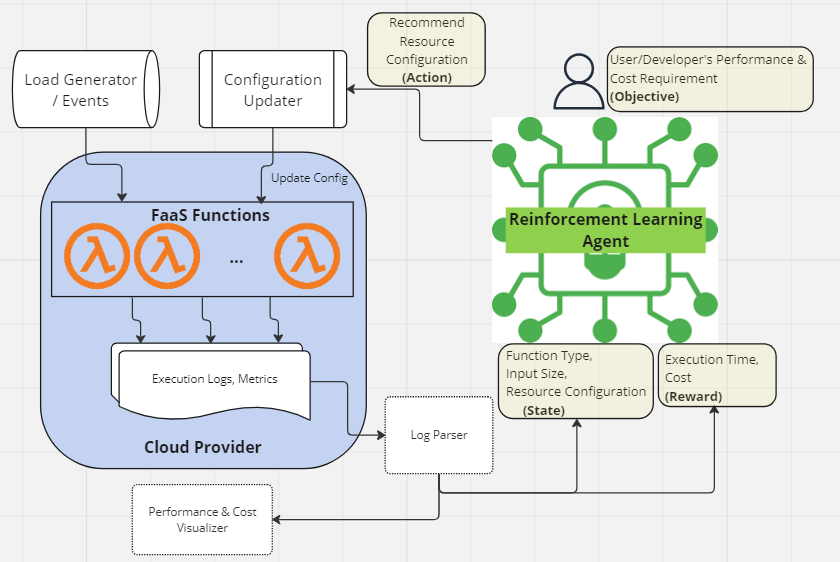
\includegraphics[width=1\linewidth]{System Architecture.PNG}
    \caption{High-level architecture of the system and the interaction
between its components in a general use case}
    \label{fig:enter-label}
\end{figure}
Other than the RL agent, there several additional component to assist with the control and feedback loop. 
\item Log Parser.

The log parser will take the output logs of FaaS function as input, and use regular expression and other methods to parse the logs, and extract useful data that will be used by the RL agent to model the function performance. These data include overall function execution time, size of the incoming request that the function receives, function type, etc. Note that the function has to implement necessary logging for this to work. The parsed data will also be fed to Performance and Cost Visualizer that allows us to monitor the agent's performance. 

\item Configuration Updater.

The Config 1 Updater will take a FaaS function and a desired memory size as input, which comes from the RL agent. It then updates the memory config 1uration of the designated FaaS function, using AWS CLI. 

\item Load Generator.

The Load generator will be responsible for generating requests of different types and in different patterns and sending these requests to the target FaaS function, which is necessary to explore the performance of the FaaS function under different memory settings.

Load Generator will also play an important part in our experimentation stage, where we need to generate and send synthetic traffic of specific trends to the FaaS applications to mimic the in-production scenario, in order to evaluate the performance of our algorithm.

The actual function/application we plan to test are listed in Table 1, following the classification of FaaS functions developed by Zhang et al. \cite{10.1007/978-3-030-96326-2_2}. Experimenting on these four functions of different type should provide a comprehensive view of how practical is our system in different area of applications.

\end{itemize}
\begin{table*}
\centering

\begin{tabular}{| l | l | l |}
\hline
Category & Description & Language \\
\hline

\hline
CPU-intensive function & Compute complex mathematical formulas using multiple threads & Python \\
\hline
Memory-intensive function & Summation of large integer arrays & Java \\
\hline
Image processing application & Image recognition & Java \\
\hline
Big data processing function & Word frequency statistics & Python \\
\hline

\end{tabular}
\caption{Four functions to Deploy and Test}
\label{tab:enter-label}
\end{table*}



\subsection{What hypothesis do you want to test?}
We would like to test three hypotheses.
\begin{itemize}
\item For a given FaaS function, the proposed framework is able to find out the optimal memory config 1uration quickly under stable workload.

Similarly, we will test both time to convergence and accuracy of our system, by sending stable workload to FaaS functions. We plan to compare the performance with a baseline method, Sizeless \cite{10.1145/3464298.3493398}, to show our method is more efficient in finding an optimal memory value.


\item With the adoption of this system, FaaS executions should comply with SLO requirements, and are able to achieve optimal/near-optimal objective.

We will implement a few types of FaaS applications, apply our framework, specify different SLO requirements, and generate synthetic traffic to the lambda functions in order to measure how well do these functions adhere to specified SLO, as an indicator of the effectiveness of our system.

\item When the incoming workload changes, the proposed framework would quickly detect and react by dynamically updating the optimal memory config 1uration, in order to ensure adherence to SLO and other objectives.
We will send requests with different sizes to the functions at different frequency, and understand how our system adjusts the recommended memory in response to varying traffic volume.
\end{itemize}

\subsection{What measurements do you intend to collect? Why \& What for?}

We plan to measure the performance of the proposed framework using a few synthetic/real-world FaaS functions. Functions would each represent a different type of common applications, for instance, network-intensive task or CPU-intensive task. We will evaluate the performance independently for each of the chosen FaaS functions. 

For each FaaS function, it will first be set up in AWS Lambda. The traffic generator will send out synthetic requests that follow a specified pattern. The proposed framework will be implemented and config 1ured to oversee this target FaaS function. 

First, without the interference from the optimization framework, the execution time and associated cost of synthetic requests will be measured at different memory sizes. This will be used as baseline data to identify the optimal memory size given user specified optimization goal.

Then, we will turn on the optimization framework and let it optimize the memory config 1uration of the target lambda function in the fly. Again, the execution time and associated cost of each of the requests will be measured, as well as the memory size that is suggested by the framework in each round. We will also track the sequence of the requests in order to monitor convergence.

For each of the three hypotheses, there will be slight differences in the system setup as well as the metrics to compare:

\begin{itemize}
\item The ability to find out the optimal memory size under stable traffic patterns, given different optimization objectives (e.g., execution time or budget).

For this hypothesis, synthetic traffic will have similar input sizes in relatively steady pace, mimicing the scenario where a service receives stable and similar requests coming in throughout the day. 

From the baseline data, we will be able to pick the optimal/suboptimal memory size, which serves as the ground truth. We then compare the final memory size that the system converges to with the ground truth, and measure how well does the system successfully find the actual optimal/sub-optimal memory sizes for each FaaS function. Specifically, we plan to measure the percentage of times the system finds the optimal memory size, as well as number of rounds it takes the system to reach a stable memory size recommendation.

\item Compliance to SLO while optimizing for other objectives.

For this hypothesis, the system setup would be the same as the previous scenario. The execution time of each request will be compared against the SLO to understand how well this system is able to comply to SLO requirement.

Given other objectives, e.g., cost, we will also collect cost for each request, and measure against baseline cost to understand the system's ability to optimize cost while adhering to SLO.


\item The ability to dynamically determine optimal memory config 1uration given changing request patterns.

Synthetic requests sent out by the traffic modeler will be conhigh-levelured to have very different patterns throughout the day, categorized into several cohorts. For instance, one cohort would have a large size of requests, potentially demanding a lambda with higher memory size to support it, while another cohort would consist of lightweight requests. 

Again, we start with collecting baseline data, i.e., execution time and cost at different memory sizes, without interference of the optimization framework. This gives us the optimal memory size for each cohort.

We then turn on optimization framework. For each cohort, we plan to measure execution time, cost, and memory size it picks for each request. We will look at the data and identify the final memory size the algorithm converges to for each cohort, and compare to the ground truth to see if the algorithm picks the right memory size dynamically for different cohorts.

Additionally, we will measure the number of rounds it takes for the algorithm to converge to the new optimal point, which demonstrates how fast it is able to adapt to traffic change.

We will also measure the percentage of requests that confirm to SLO in this scenario, as an extra piece of evidence of the SLO adherence.

\end{itemize}


\subsection{What will a successful outcome look like?}
For each of the three hypotheses, a successful outcome should look like:
\begin{itemize}
%TODOTODOTODO
\item The ability to find out the optimal memory size under stable traffic patterns, given different optimization objectives (e.g., execution time or budget).

In this experiment, we expect to see that the converged memory size proposed by the framework is the same as the actual optimal memory size from the ground truth data, for all FaaS functions that we test. Additionally, we expect to see that it only takes a small number of iterations of memory conhigh-levels before the algorithm makes a convergence, indicating that the algorithm is able to quickly find the optimum.

\item Compliance to SLO, while optimizing for other objectives.

The first experiment looks at how well the algorithm optimizes for a given objective. In this experiment, we want to validate that the algorithm is able to adhere to the specified SLO. We expect to see that with the proposed optimization framework, there is a high percentage of requests with execution times below SLO threshold. 

\item The ability to dynamically determine optimal memory conhigh-leveluration given changing request patterns.

We expect to see that once the pattern of input requests changes, the algorithm takes only a small number of requests to find out the new optimal memory size. This reflects how quickly the algorithm is able to dynamically find optimal memory configurations. Throughout the experiment, we also expect to see a high percentage of requests conforming to SLO while the pattern of input requests changes once in a while.

\end{itemize}


% \section{Preliminary experimental results or proof of concept}

% Any preliminary experimental results or proof of concept at this stage is a plus but not required... Unlikely we would submit this section for M2 so commented out for now



\bibliographystyle{IEEEtran}
\bibliography{refs}

\end{document}
